\begin{figure}[htbp]
    \centering

    \begin{minipage}{0.24\textwidth}
        \centering
        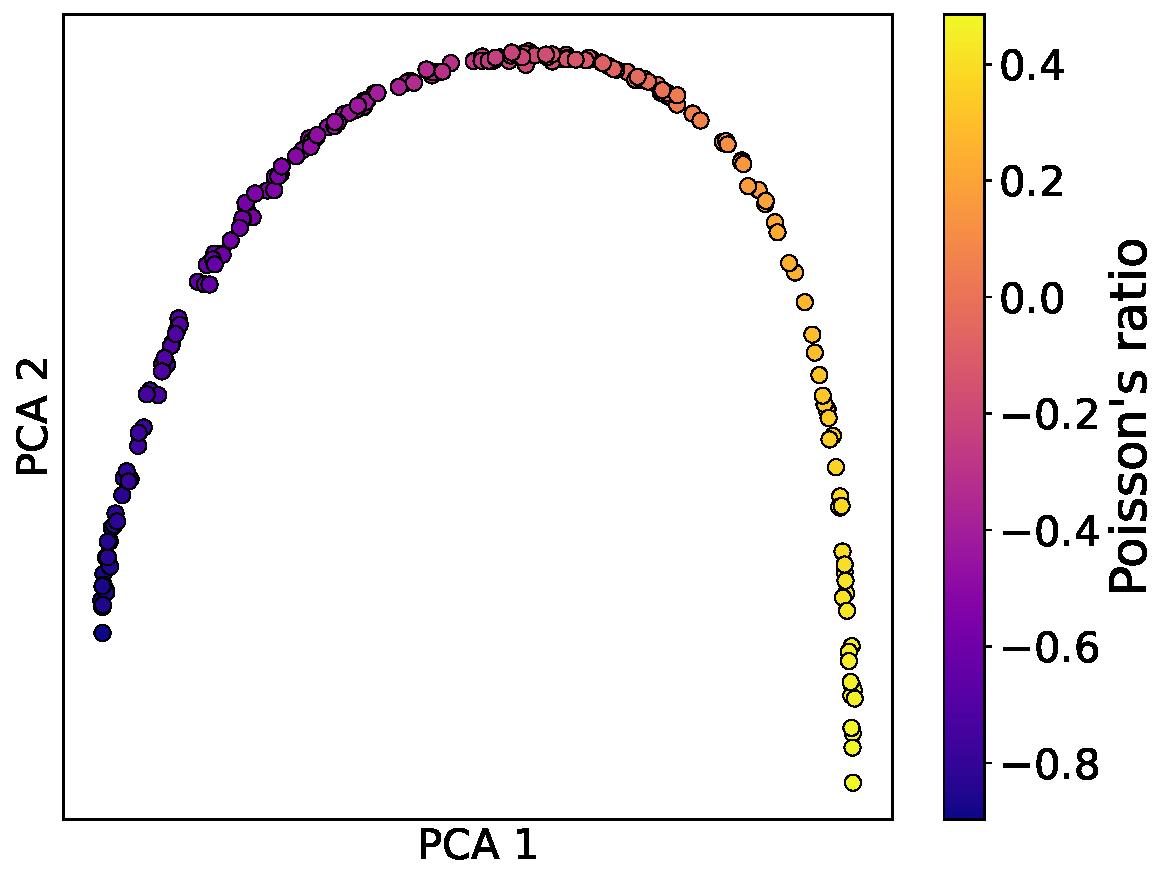
\includegraphics[width=\textwidth]{figures/latent_space_vis/pca_peach_db_poisson.pdf}\\
        {\small \hspace{-1mm}\texttt{Deforming Block}}
    \end{minipage}
    \begin{minipage}{0.24\textwidth}
        \centering
        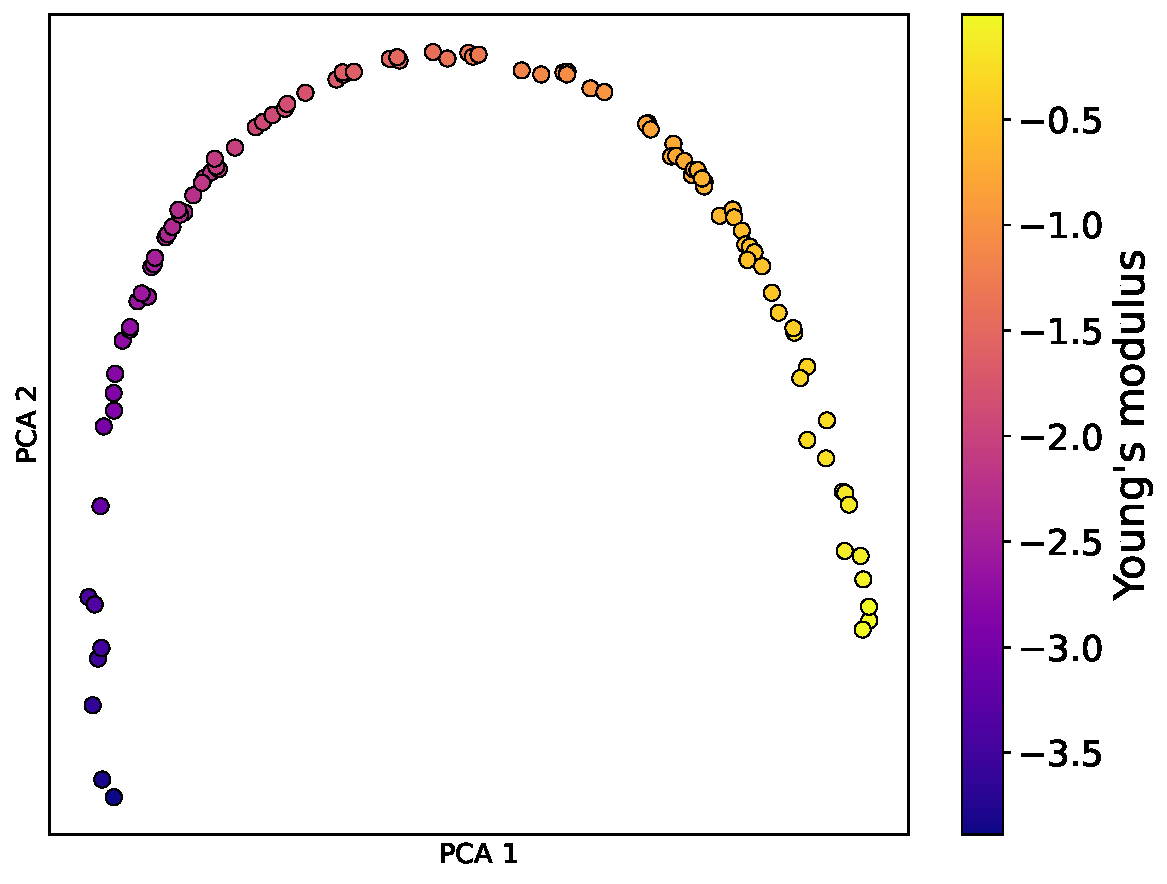
\includegraphics[width=\textwidth]{figures/latent_space_vis/pca_peach_sd_young_modulus.pdf}\\
        {\small \hspace{-2mm}\texttt{Sheet Deformation}}
    \end{minipage}
    \begin{minipage}{0.24\textwidth}
        \centering
        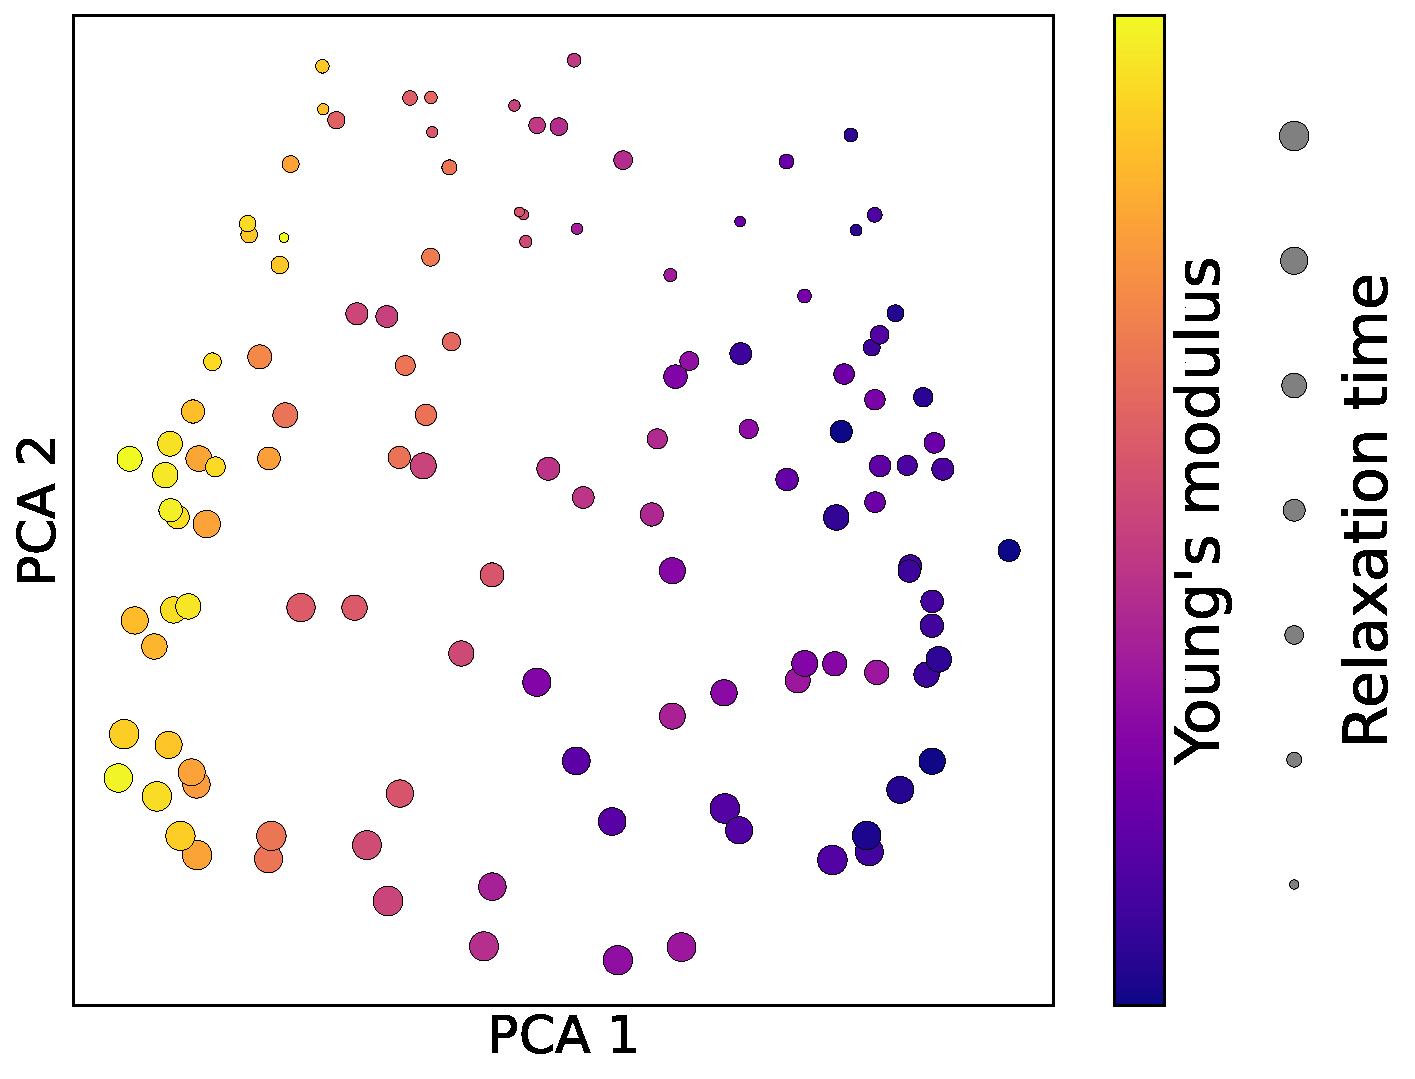
\includegraphics[width=\textwidth]{figures/latent_space_vis/pca_peach_bbv_bivariate.pdf}\\
        {\small \hspace{-1mm}\texttt{Bending Beam}}
    \end{minipage}
    \begin{minipage}{0.24\textwidth}
        \centering
        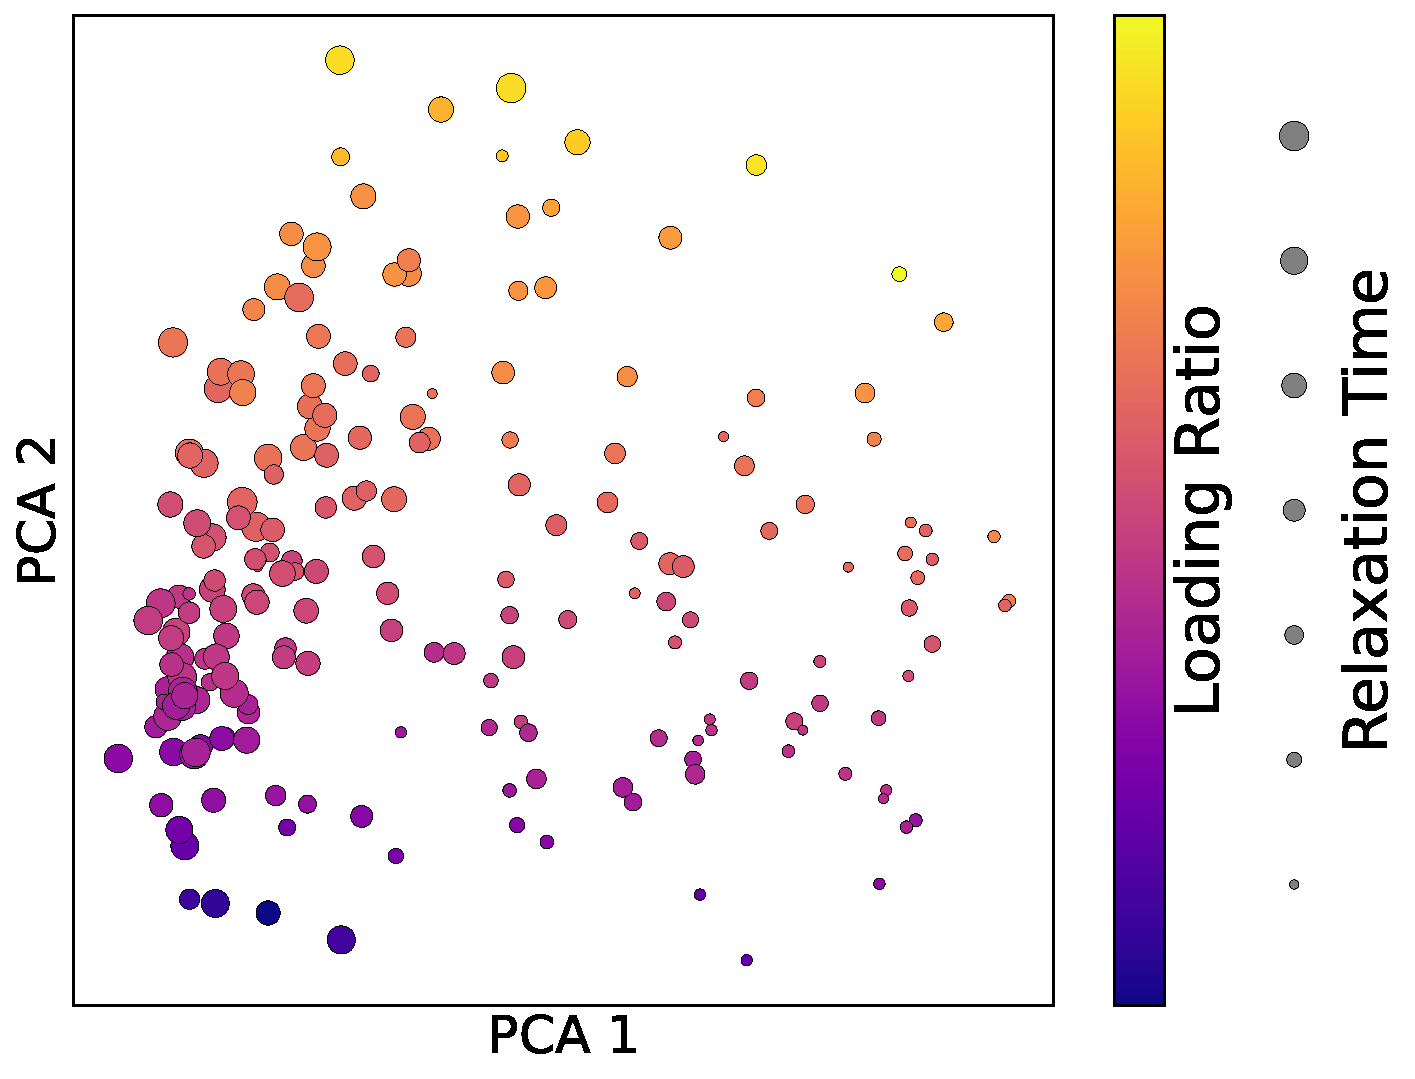
\includegraphics[width=\textwidth]{figures/latent_space_vis/pca_peach_trampoline_bivariate.pdf}\\
        {\small \hspace{-2mm}\texttt{Trampoline}}
    \end{minipage}

    \caption{
        PCA visualization of the latent space on the Deforming block, Sheet deformation, Bending beam and Trampoline environment (left to right).
        Each point represents an encoded task, with different coloring and scaling references based on the task's material properties.
    }
    \label{fig:latents_appendix}
\end{figure}